\documentclass{sig-alternate-05-2015}
\usepackage{caption}

\begin{document}
\toappear

\title{Analysis of Zstandard, a fast and modern compression algorithm}

\numberofauthors{1} %  in this sample file, there are a *total*
\author{
\alignauthor
Charles Vandevoorde\\
       \affaddr{Computer science master student at ECAM}\\
       \affaddr{Promenade de l'Alma, 50}\\
       \affaddr{Woluwe-Saint-Lambert, Belgium}\\
       \email{13019@student.ecam.be}
}

\maketitle

\begin{abstract}
    Compression algorithms are used everywhere in modern computing: database, web assets, \ldots
    This paper analyses a new compression algorithm presented this year by a team at
    \textit{Facebook}. First, we will analyse how the compression algorithm works then we will study
    how a compressed document is formatted in file. Finally, we will see how Zstandard arrive at
    such good compression ratio with a great speed. The speed is mostly due to the use of modern
    CPU capability and the compression ratio is due to new research in prefix coding and to the
    adaptation of the algorithm to modern computer.

\end{abstract}

\keywords{Compression; Performance; Zstandard}

\section{Introduction}
    Data are a major piece in modern computing. Companies have to share, store and back up a
    lot of information. Lossless compression algorithm allow them to reduce the cost of servers and
    cut down bandwidth. The most common general purpose algorithm for data compression nowadays is
    deflate with his known implementation zlib.  This library has been around for nearly two decades
    and no others algorithms could reach a ratio speed and space that balanced. Using modern
    technology, a \textit{Facebook} team happen to get a way better time and space ratio with their
    new algorithm Zstandard. I will demonstrate how Zstandard comes to this performance using modern
    hardware properties and new algorithm research.

\section{Compression algorithm \\ explained}
    Zstandard use a very similar technique to the deflate compression algorithm. First, duplicated
    bit sequences are found in the sliding window. The sliding window is a bounded record of
    previous uncompressed data.  The first bit sequence is written as a sequence of literal bits.
    Following duplicated bit sequences are expressed as an offset refering the literal, the
    lenght of this literal and a copy lenght. The copy command take the matched
    literal and copy it until the copy lenght is fulfilled. This operation is called \textit{match
    and copy}.

    Zstandard uses also another well known compression algorithm, the run-lenght encoding algorithm
    (also known as RLE). This algorithm replace a repeating sequence with the lowest common
    denomitor of the sequence and with the total lenght of the repeating sequence. With this two
    information, Zstandard can regenerate the repeating sequence.

    Secondly, Zstandard uses a method called entropy encoding to reduce the number of bits needed to
    encode a literal. An entropy encoder use the occurence probability of literals to generate
    specifics prefixes codes. A prefix code is a word code with the property that no others words
    codes have the same prefix. Prefix code can thus create literals with varying lenght. Those
    specifics prefixes codes have their lenghts inversely proportional to their occurences
    probabilities reducing lenght of common literals and increasing the lenght for rares one. The
    average lenght can therefore be reduced. Information from \textit{match and copy} operations can
    also be encoded to reduce the compressed size further. A widely known entropy encoder is the
    Huffman encoder used in the deflate algorithm. Zstandard uses Huff0 and FSE as entropy coder.

    \subsection{Entropy coder}
    \subsubsection{Huff0}
        Huff0 is an implementation of an Huffman coder. This implementation is faster than the
        zlib one because it uses some optimisations discussed in Section \ref{sec:perf}.

        The huffman algorithm creates a binary tree structure from the bottom up where the hightest
        weight (number of occurence of a sequence) is on top and the lowest weight are on the
        bottom. If the left and right edges have respective value of 0 and 1, a prefix code can be
        defined for each sequence with his bit lenght inversely proportional to his occurence
        probability.

    \subsubsection{Finite state entropy}
        Finite state entropy \cite{fse} is an arithmetic coder based on ANS theory \cite{ANS2013}.
        Arithmetic coder have an entropy close to the Shannon limit which is the optimal size that a
        probability can be encoded. This entropy can be achieved because high probability sequence
        can be encoded with less than a bit. The main drawback is massive usage of multiplication
        and division which can be very slow. FSE use a modified version of the arithmetic coder that
        doesn't use any multiplications and divisions but only additions, shifts and tables lookups. The
        functioning of this algorithm will not be discussed here because of his complexity.

\section{Compression format}
    A compressed file with Zstandard \cite{compress_format} is a set of frames. Frames are
    independant parts containing some parameters and blocks which contains the compressed data. As
    frames are independents, data can be added to the compressed file without recompress everything by
    appending a new frame at the end of the compress file. Frame parameters are for exemple a
    checksum for validating the information, the size of the sliding window, a dictionnary ID if we
    use one and some others parameters giving the existing parameters and multiples sizes for the
    decoder.

    A block contains a flag to tell if it is the last block of the frame, a block type flag, the
    block size and then the block content. A block can have differents types such as RLE blocks,
    Zstandard compressed blocks or raw blocks. A block has a 128 KB maximum size; but if the sliding
    window is lesser than the maximum size, the block has a max size equal to the sliding window.

    The Zstandard compressed block is composed of a literals section and a sequences section. The
    literals section represent the data that will be used for the \textit{match and copy} operation.
    The sequences section is a representation of the \textit{match and copy operation} that give the
    lenght of the literal to copy, the offset and a reconstruction lenght. The offset gives the
    relative position of the previous block. When all the sequences of a block are decoded, if there is
    unused literal, these bytes will be copied at the current position in the decompressed file. A
    block can also contains an Huffman tree giving the prefix code translation.

    The literals section can be encoded using the Huff0 for more speed or FSE for less size but the
    sequences sections are forced to use the FSE encoding. Of course, those sections can also not be
    encoded to gain more speed or because it doesn't improve the compression ratio.

\section{Comparaison over deflate}
    \begin{figure}
        \centering
        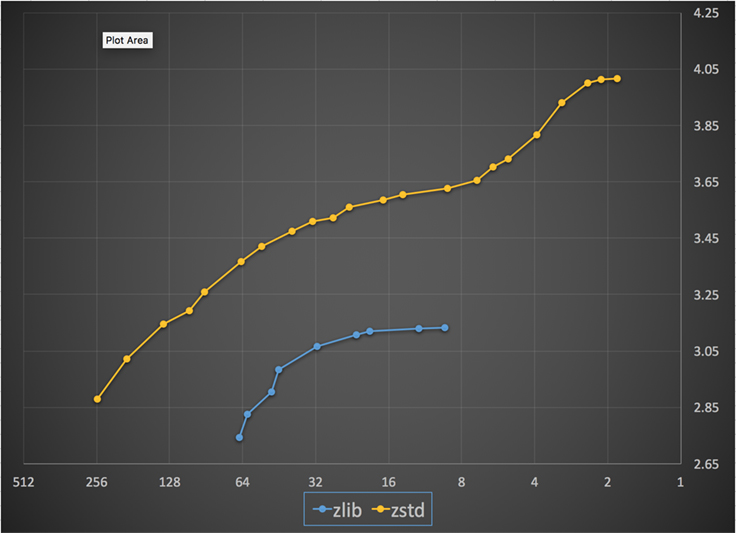
\includegraphics[scale=0.5]{speed.jpg}
        \caption{Comparaison between compression levels for zstd and zlib}
        \label{fig:level}
    \end{figure}
    \begin{figure}
        \centering
        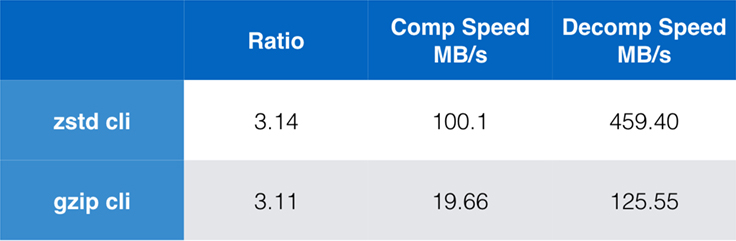
\includegraphics[scale=0.25]{speed_comp.jpg}
        \caption{Comparaison between compression and decompression speed between zstd and gzip
        (default compression level)}
        \label{fig:speed}
    \end{figure}
    First of all, Zstandard can compress and decompress at a way bigger speed than
    deflate's implementation with a bigger compression ratio. This improvement can be seen on Figures
    \ref{fig:level} and \ref{fig:speed}. These performances improvements will be discussed in section
    \ref{sec:perf}. In Figure \ref{fig:level}, we can see that we have much more compression levels
    making Zstandard much more scalable for any given application. Those levels are achieved by
    modifying the sliding window size, the data encoding and the compression type of each frame's
    blocks.

    Another important feature is the ability to compress small data with a good ratio using
    dictionnaries \cite{dictionnary}. Small data are difficult to decompress because we don't have
    much history to work on. A dictionnary is a list of commonly used sequences and must be
    specifics for a given filetype or data format. Dictionnary compression improve the compression
    ratio from 150\% to nearly 500\% with data varying from 20 to 800KB \cite{dictionnary}.
    Zstandard intregrates directly a tool to create those dictionnary with some data samples. Of
    course, the decompression process will also need to have this dictionnary.

    \subsection{Performance}\label{sec:perf}
    \subsubsection{Memory}
        Zstandard can use up to terabytes of memory for some levels but also less than 1Mb of memory
        for the first level \cite{presentation}. It allows Zstandard to run on huge datacenter and on
        embedded environments with limited ressources. Memory play a role in the compression ratio
        because more memory means a bigger sliding window and a bigger use of past data.

    \subsubsection{Parallel excecution}
        Today's CPU can execute multiples instructions in one cycle thanks to multiple hardware
        optimisations. Superscalar CPU \cite{superscalar} executes several instructions in one cycle
        by dispatching these instructions onto differents execution units as ALU, FPU, \ldots{}
        Another feature used is the out-of-order execution \cite{outoforder}. A processor using this
        technique will dynamically reorganize the order of the instructions by data avaibility. The
        instructions must be independant for the out-of-order technique to work. To work with these
        feature, Zstandard must have data with few dependencies. The compression format include a
        mode where litteral are cut into four streams with no dependencies with each others.

    \subsubsection{Branchless design}
        New CPU use a technique called instruction pipelining \cite{pipelining}. An instruction can be
        cut in differents parts for exemple fetch, decode and execute. A simple approach would be to
        execute the first part, then the second, \ldots{} A more optimazed approach would use an
        "assembly line" like methodology. Each instruction part can be executed in a different
        portion of the CPU and then passed to the following portion so three differents instructions
        parts can be decoded in the same cycle instead of one. This method gives us a huge speed
        improvement without increasing the clock speed.

        Modern CPU use also another trick to be faster; the branch prediction. A branch can be seen
        as a \textit{if-else} statement. When the processor is waiting for the conditionnal jump
        instruction to be executed, the CPU can gamble on which branch will be correct allowing to
        move forward in the program's instructions. If the branch is the correct one, the CPU
        continue with his lead but if the branch is not correct, the CPU have to play back the
        instructions and execute the other branch. The problem with branch prediction is when we
        have also instruction pipelining, because the pipeline has to be cleared before restarting.
        Instruction pipelining clearing takes a lot of time for a modern CPU as shown on Figure
        \ref{fig:costop}. Zstandard uses what is called branchless design in critical section to
        avoid this instruction pipeline flush. Branchless code is a code where there isn't any
        branch i.e. \textit{if-else}, \textit{while/for loops}, \ldots

        \begin{figure}
            \centerline{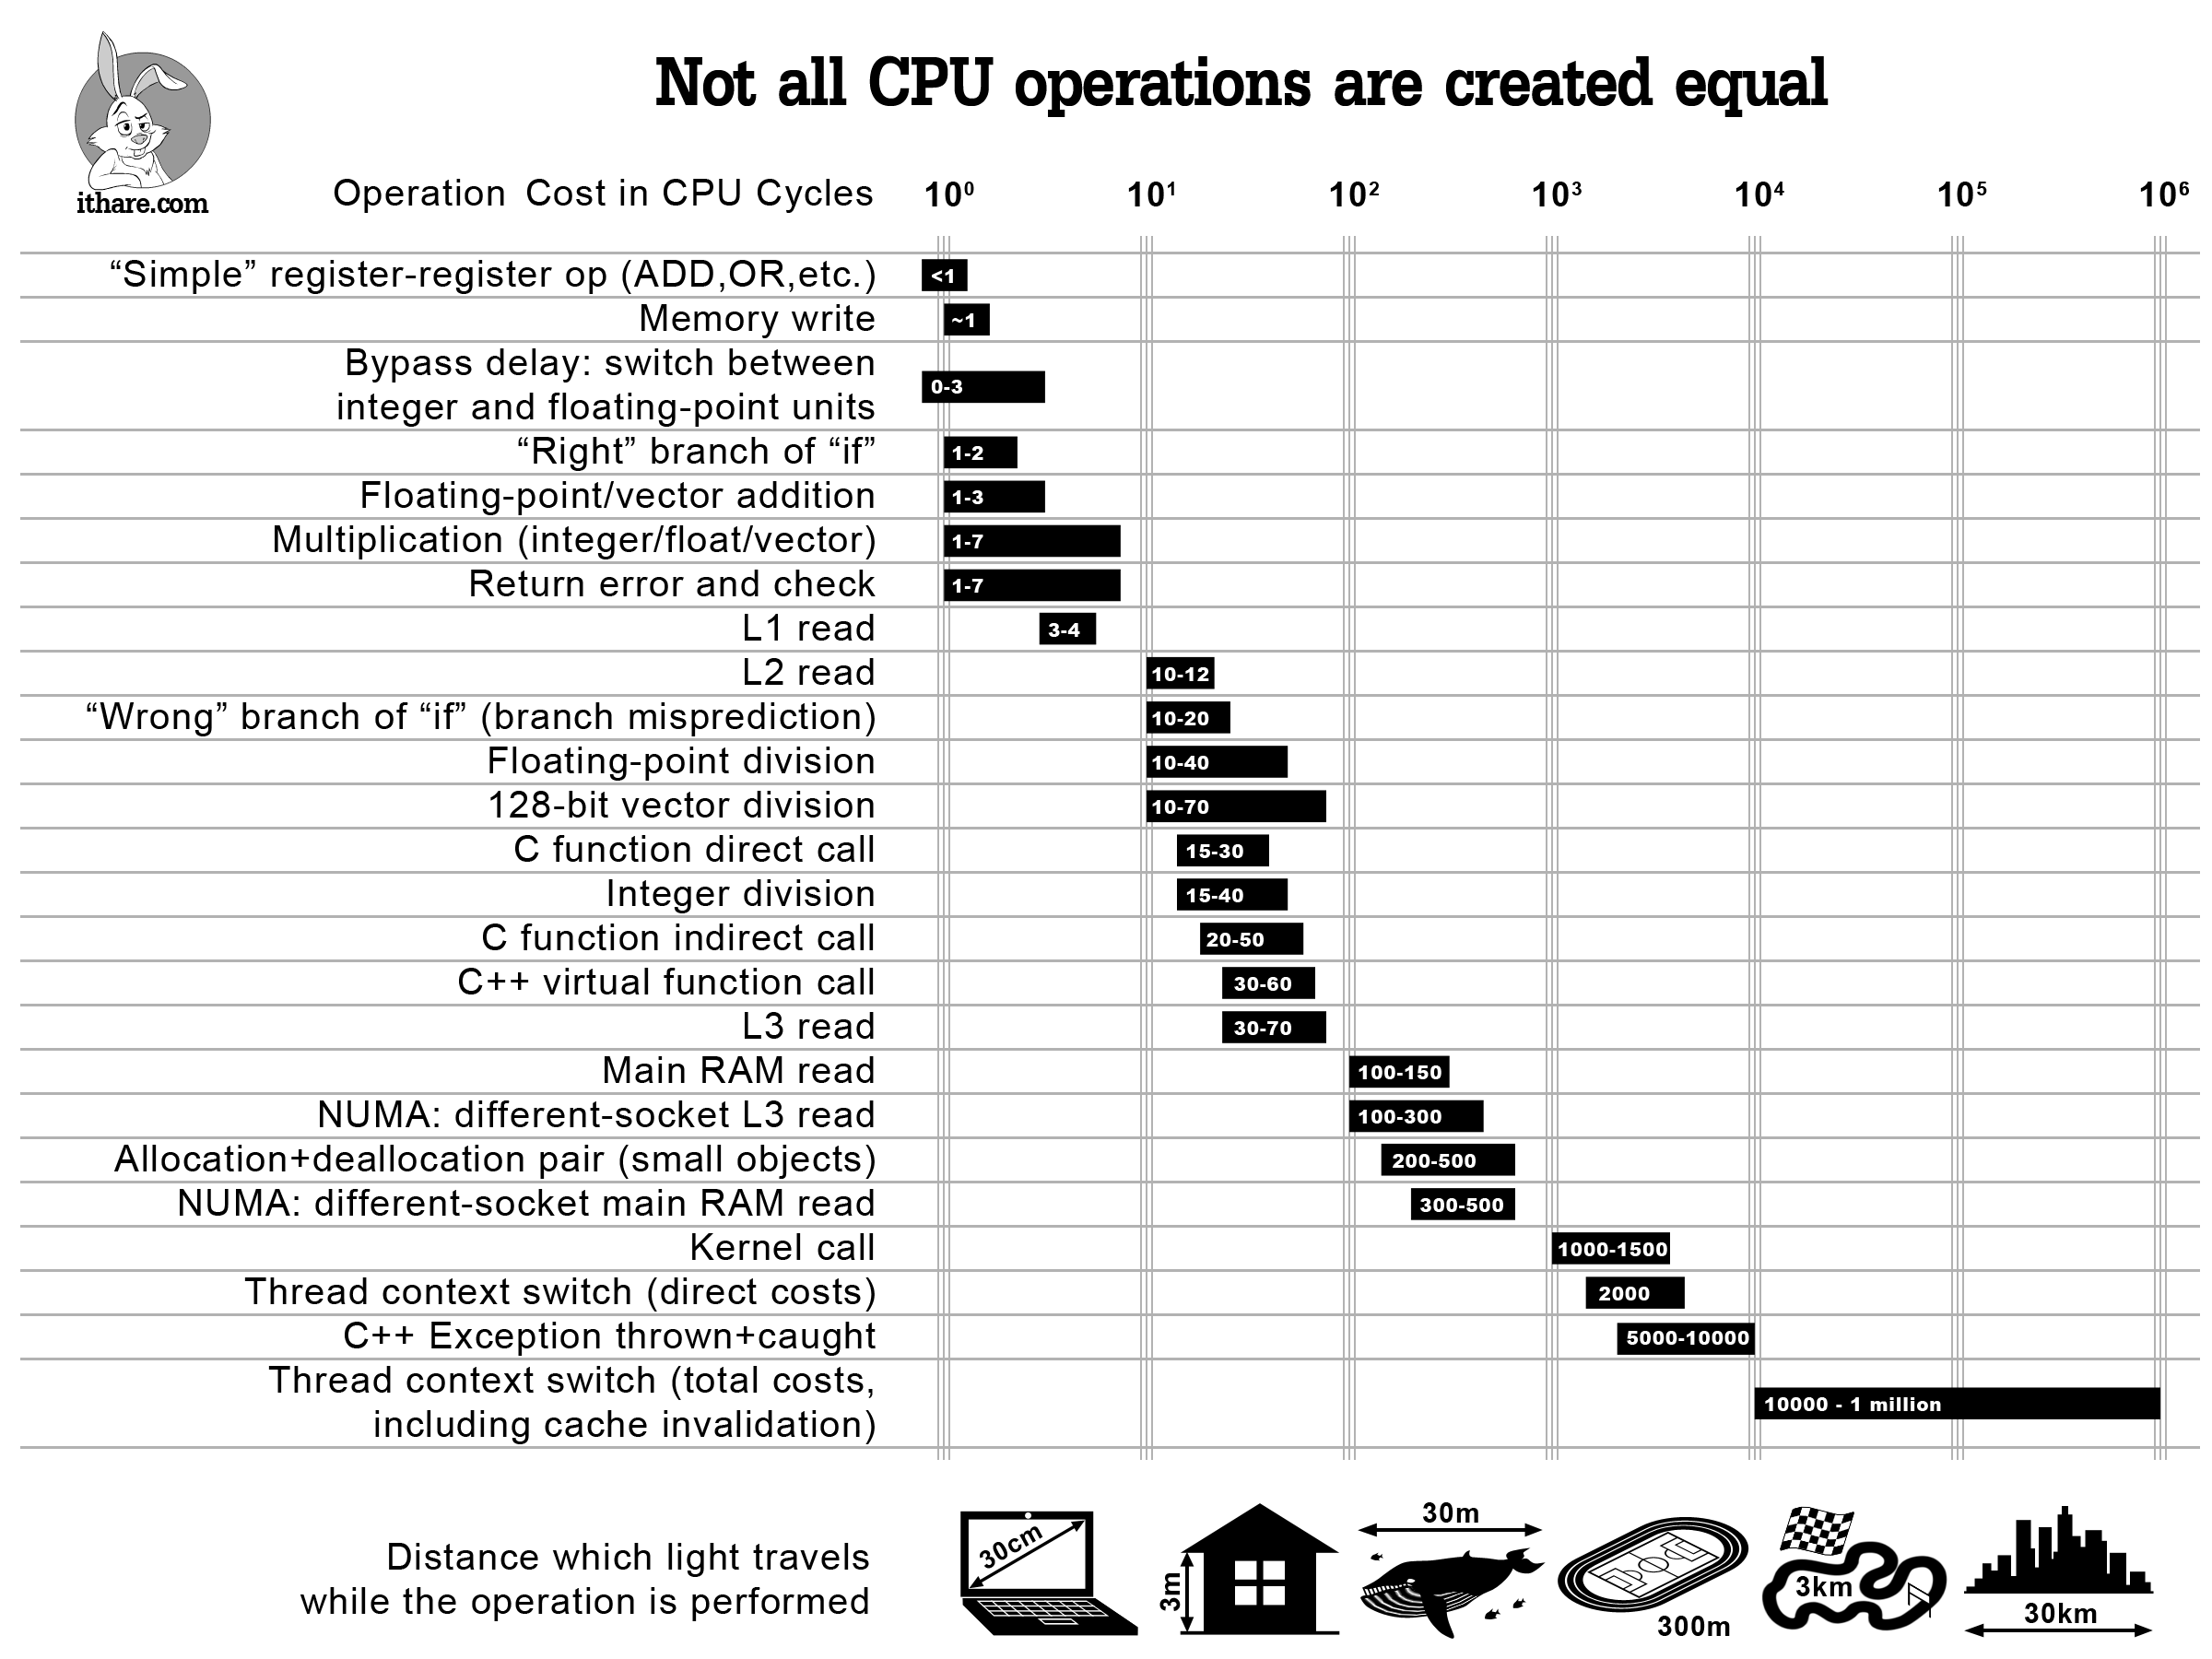
\includegraphics[scale=0.11]{costCPUop.png}}
            \caption{Operation cost per CPU cycle (Scale is logarithmic).}
            \label{fig:costop}
        \end{figure}

\section{Conclusions}
    In this paper, we highlighted the importance of well-knowing the architecture of a computer and
    how computer components are working below all the abstractions given by the OS and the
    programming language. We can see that the Zstandard team try to use every bit of optimisations
    possible which is very important in a CPU heavy application like compression.

\newpage
\bibliographystyle{unsrt}
\bibliography{biblio}  % sigproc.bib is the name of the Bibliography in this case
\end{document}
